%!TEX root = SysSpec_ClockPendulumAnalyzer.tex
\subsection{Sequenzdiagramm}
In diesem Kapitel werden einzelne Arbeitsabläufe anhand eines Sequenzdiagrammes dargestellt.
	\subsubsection{Speichern einer Datenmessung}
    Dieses Sequenzdiagramm (Abbildung \ref{fig:sequence_save}) zeigt den Ablauf zum Speichern einer Messdatenreihe. Das ganze läuft in einer endlosen Schlaufe und versucht vor einem Speichern in die Datenbank 5 Daten Samples über den \iic\ zu erhalten.
    \begin{figure}[H]
        \centering
        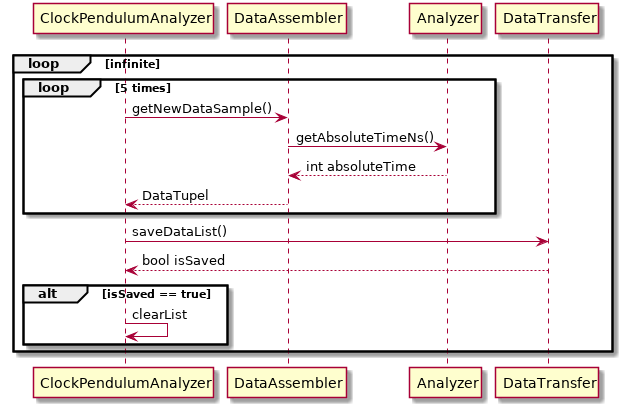
\includegraphics[width=\textwidth]{sequence_data_save.png}
        \caption{Sequenzdiagramm zum Speichern der Daten}
        \label{fig:sequence_save}
    \end{figure}

    \clearpage
    \subsubsection{Abrufen einer Datenmessung}
    Der Webclient ruft Daten über eine HTTP Request auf die angebotene REST Schnittstelle. Dabei werden folgende Sequenzen (siehe Abbildung \ref{fig:sequence_get}) abgearbeitet.
    \begin{figure}[H]
        \centering
        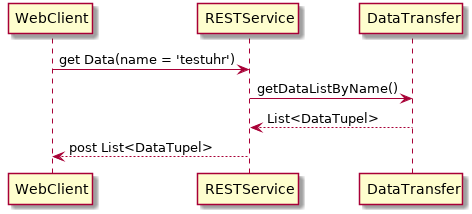
\includegraphics[width=.7\textwidth]{sequence_data_access.png}
        \caption{Sequenzdiagramm zum Aufrufen der Daten}
        \label{fig:sequence_get}
    \end{figure}